\documentclass{article}

\usepackage{graphicx,amsmath}

\title{Problem4 Report}
\author{Qi Liu}
\date{\today}

\begin{document}

\maketitle

\section{Mean Filter}
This section we will talk about the mean filters, including arithmetic mean filter $$\hat{f}(x,y)=\frac{1}{mn}\sum_{(s,t)\in S_{xy}}g(s,t),$$ geometric mean filter $$\hat{f}(x,y)=[\prod_{(s,t)\in S_{xy}}g(s,t)]^{\frac{1}{mn}},$$ harmonic mean filter $$\hat{f}(x,y)=\frac{mn}{\sum\limits_{(s,t)\in S_{xy}}\frac{1}{g(s,t)}}$$ and contra-harmonic mean filter $$\hat{f}(x,y)=\frac{\sum\limits_{(s,t)\in S_{xy}}g(s,t)^{Q+1}}{\sum\limits_{(s,t)\in S_{xy}}g(s,t)^Q}.$$

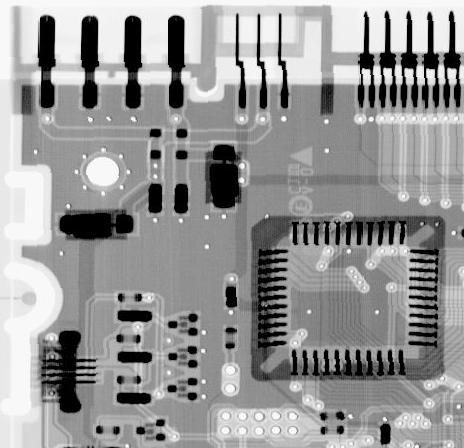
\includegraphics[width=0.25\textwidth]{../data/Circuit.jpg}
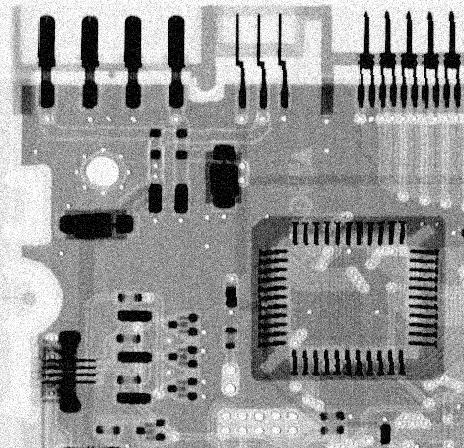
\includegraphics[width=0.25\textwidth]{../data/gauss_Circuit.jpg}
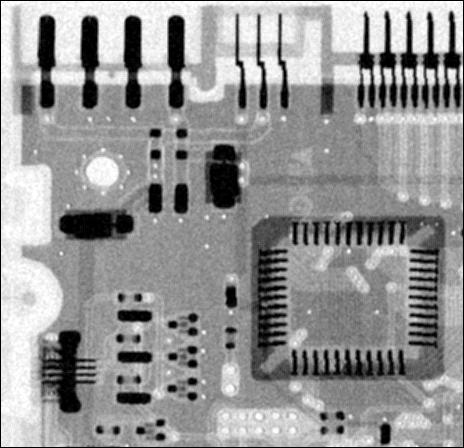
\includegraphics[width=0.25\textwidth]{../data/arithmetic_mean_gauss_Circuit.jpg}
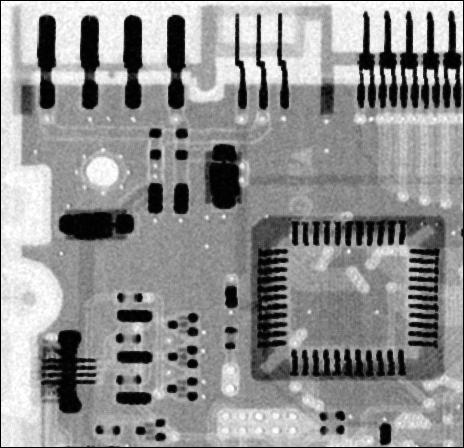
\includegraphics[width=0.25\textwidth]{../data/geometric_mean_gauss_Circuit.jpg}

The first image is the original one. The second one is corrupted by additive Gaussian noise with 0 mean and 400 variance. The third and the fourth images are the results of 3 order arithmetic mean filter and 3 order geometric mean filter.
We can see they both reduce the noises but arithmetic mean filter blurred the image more than geometric mean filter.

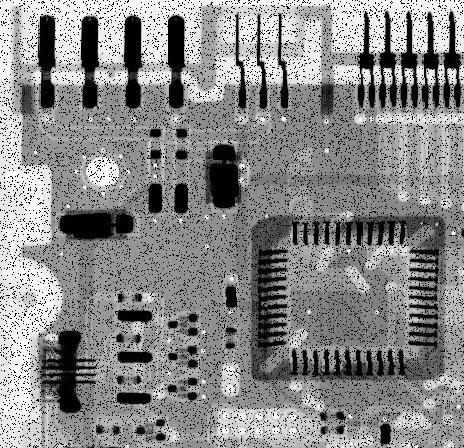
\includegraphics[width=0.25\textwidth]{../data/pepper_Circuit.jpg}
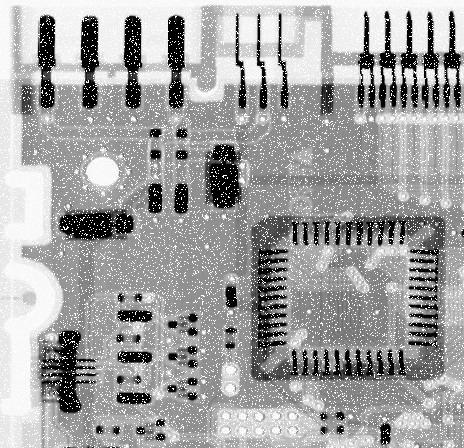
\includegraphics[width=0.25\textwidth]{../data/salt_Circuit.jpg}
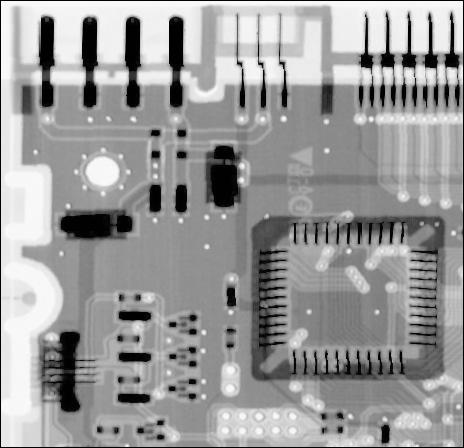
\includegraphics[width=0.25\textwidth]{../data/contra_harmonic_mean_pepper_Circuit.jpg}
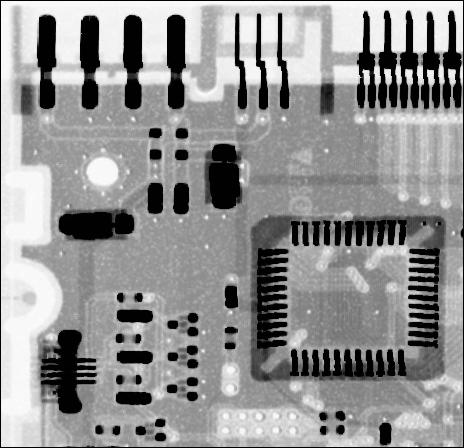
\includegraphics[width=0.25\textwidth]{../data/contra_harmonic_mean_salt_Circuit.jpg}

The first image is corrupted by pepper noise with probability 0.1. The second one is corrupted by salt noise with the same probability. The third and the fourth images are the results of 3 order contra-harmonic filter with $Q=1.5$ working on pepper image and $Q=-1.5$ working on salt image, respectively. We can see the results are reasonable.

\section{Order Statistic Filter}
This section we will talk about the order statistic filters, including median filter $$\hat{f}(x,y) = \underset{(s,t)\in S_{xy}}{\mathrm{median}}\{g(s,t)\},$$ max filter $$\hat{f}(x,y)=\max\limits_{(s,t)\in S_{xy}}\{g(s,t)\},$$
min filter $$\hat{f}(x,y)=\min\limits_{(s,t)\in S_{xy}}\{g(s,t)\},$$ midpoint filter $$\hat{f}(x,y)=\frac{1}{2}[\max\limits_{(s,t)\in S_{xy}}\{g(s,t)\}+\min\limits_{(s,t)\in S_{xy}}\{g(s,t)\}],$$ and alpha-trimmed mean filter $$\hat{f}(x,y)=\frac{1}{mn-d}\sum_{(s,t)\in S_{xy}}g_r(s,t).$$

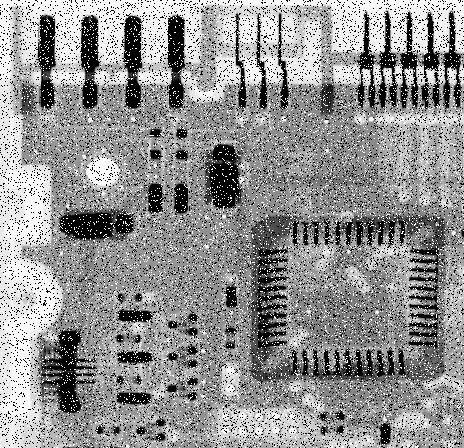
\includegraphics[width=0.33\textwidth]{../data/pepper_salt_Circuit.jpg}
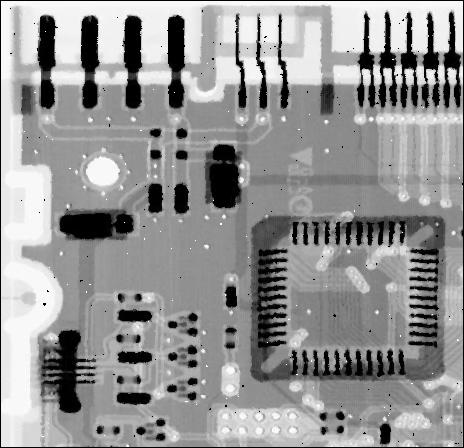
\includegraphics[width=0.33\textwidth]{../data/median_pepper_salt_Circuit.jpg}
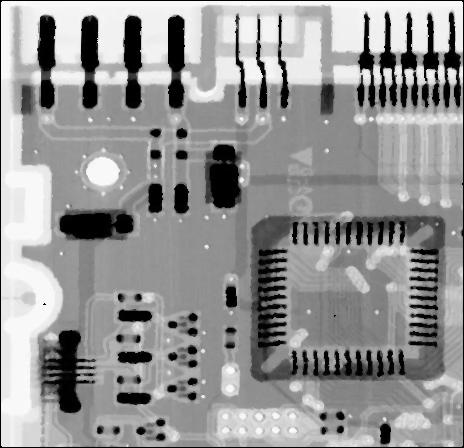
\includegraphics[width=0.33\textwidth]{../data/median_median_pepper_salt_Circuit.jpg}

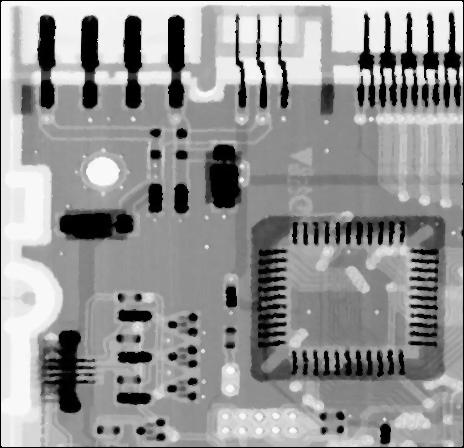
\includegraphics[width=0.33\textwidth]{../data/median_median_median_pepper_salt_Circuit.jpg}
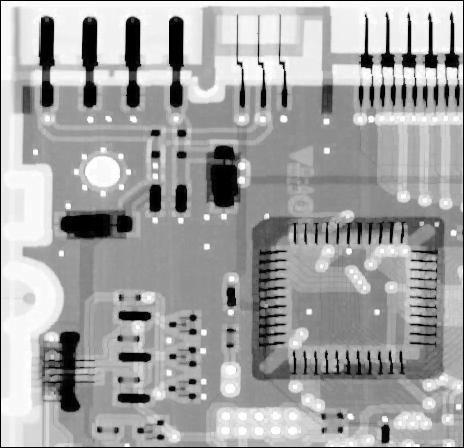
\includegraphics[width=0.33\textwidth]{../data/max_pepper_Circuit.jpg}
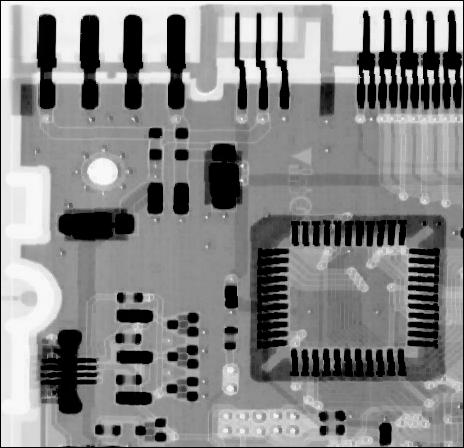
\includegraphics[width=0.33\textwidth]{../data/min_salt_Circuit.jpg}

The first image is corrupted by pepper and salt noises with probability 0.1 respectively. The second image is the result of mean filter. We can still see some noises. The third image is the result of using mean filter twice, almost every noise has been removed. The fourth image is the result of using mean filter three times, we can hardly find any noises. The fifth and the sixth images are the results of max filter working on pepper noises and min filter working on salt noises.

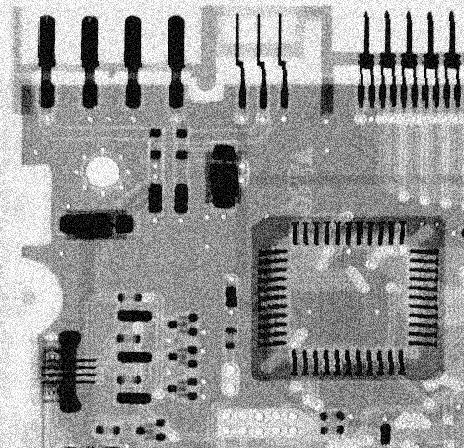
\includegraphics[width=0.33\textwidth]{../data/uniform_Circuit.jpg}
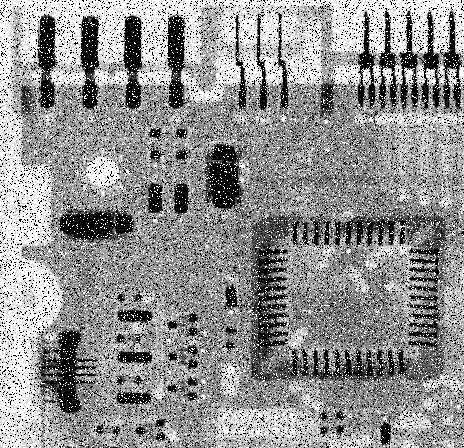
\includegraphics[width=0.33\textwidth]{../data/uniform_pepper_salt_Circuit.jpg}
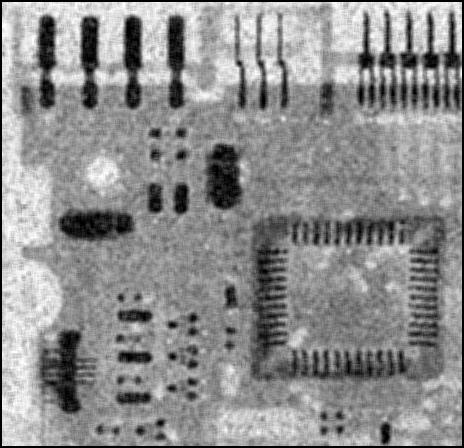
\includegraphics[width=0.33\textwidth]{../data/arithmetic_mean_uniform_pepper_salt_Circuit.jpg}

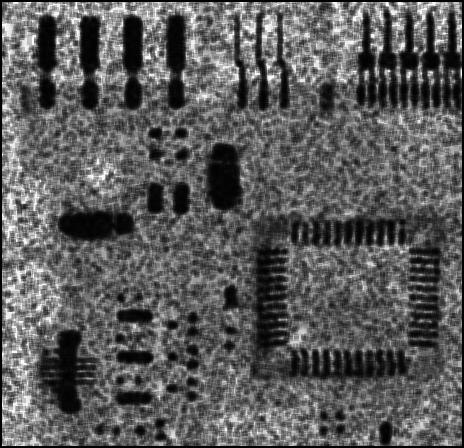
\includegraphics[width=0.33\textwidth]{../data/geometric_mean_uniform_pepper_salt_Circuit.jpg}
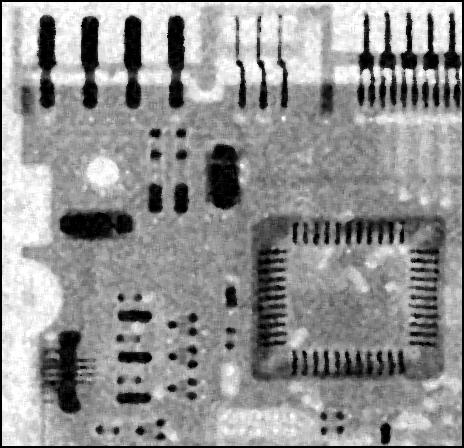
\includegraphics[width=0.33\textwidth]{../data/median_uniform_pepper_salt_Circuit.jpg}
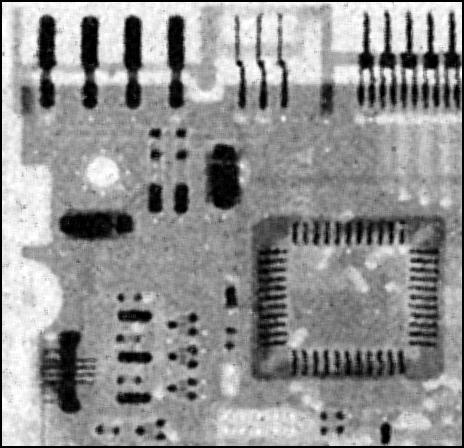
\includegraphics[width=0.33\textwidth]{../data/alpha_trimmed_mean_uniform_pepper_salt_Circuit.jpg}

The first image is corrupted by additive uniform noise with 0 mean and 800 variance. The second is corrupted more by pepper and salt noises with probability 0.1 respectively. The third and the fourth images are the results of 5 order arithmetic mean filter and geometric mean filter. We can see they are not good especially the geometric mean filter. The fifth and the sixth images are the results of 5 order median filter and alpha-trimmed mean filter with $d=5$, we can see they produce pretty good performance.

\end{document}